
% Preamble
\documentclass[11pt,a4paper]{article}
\usepackage{amsmath,amssymb}
\usepackage[dutch]{babel}

\usepackage{graphicx}

\title{Mijn derde \LaTeX\ document}
\author{Arno Kuijlaars}
\date{11 oktober 2023}

% Body
\begin{document}
\maketitle

\section{PDF file inlezen}
De Airyfunctie wordt gegeven door de formule
\[ \text{Ai}(x) = \frac{1}{\pi} \int_0^{\infty} \cos \left( \frac{t^3}{3} + xt\right) dt
\]
Let op dat dit een oneigenlijke integraal is.

\begin{figure}[h]
\centering
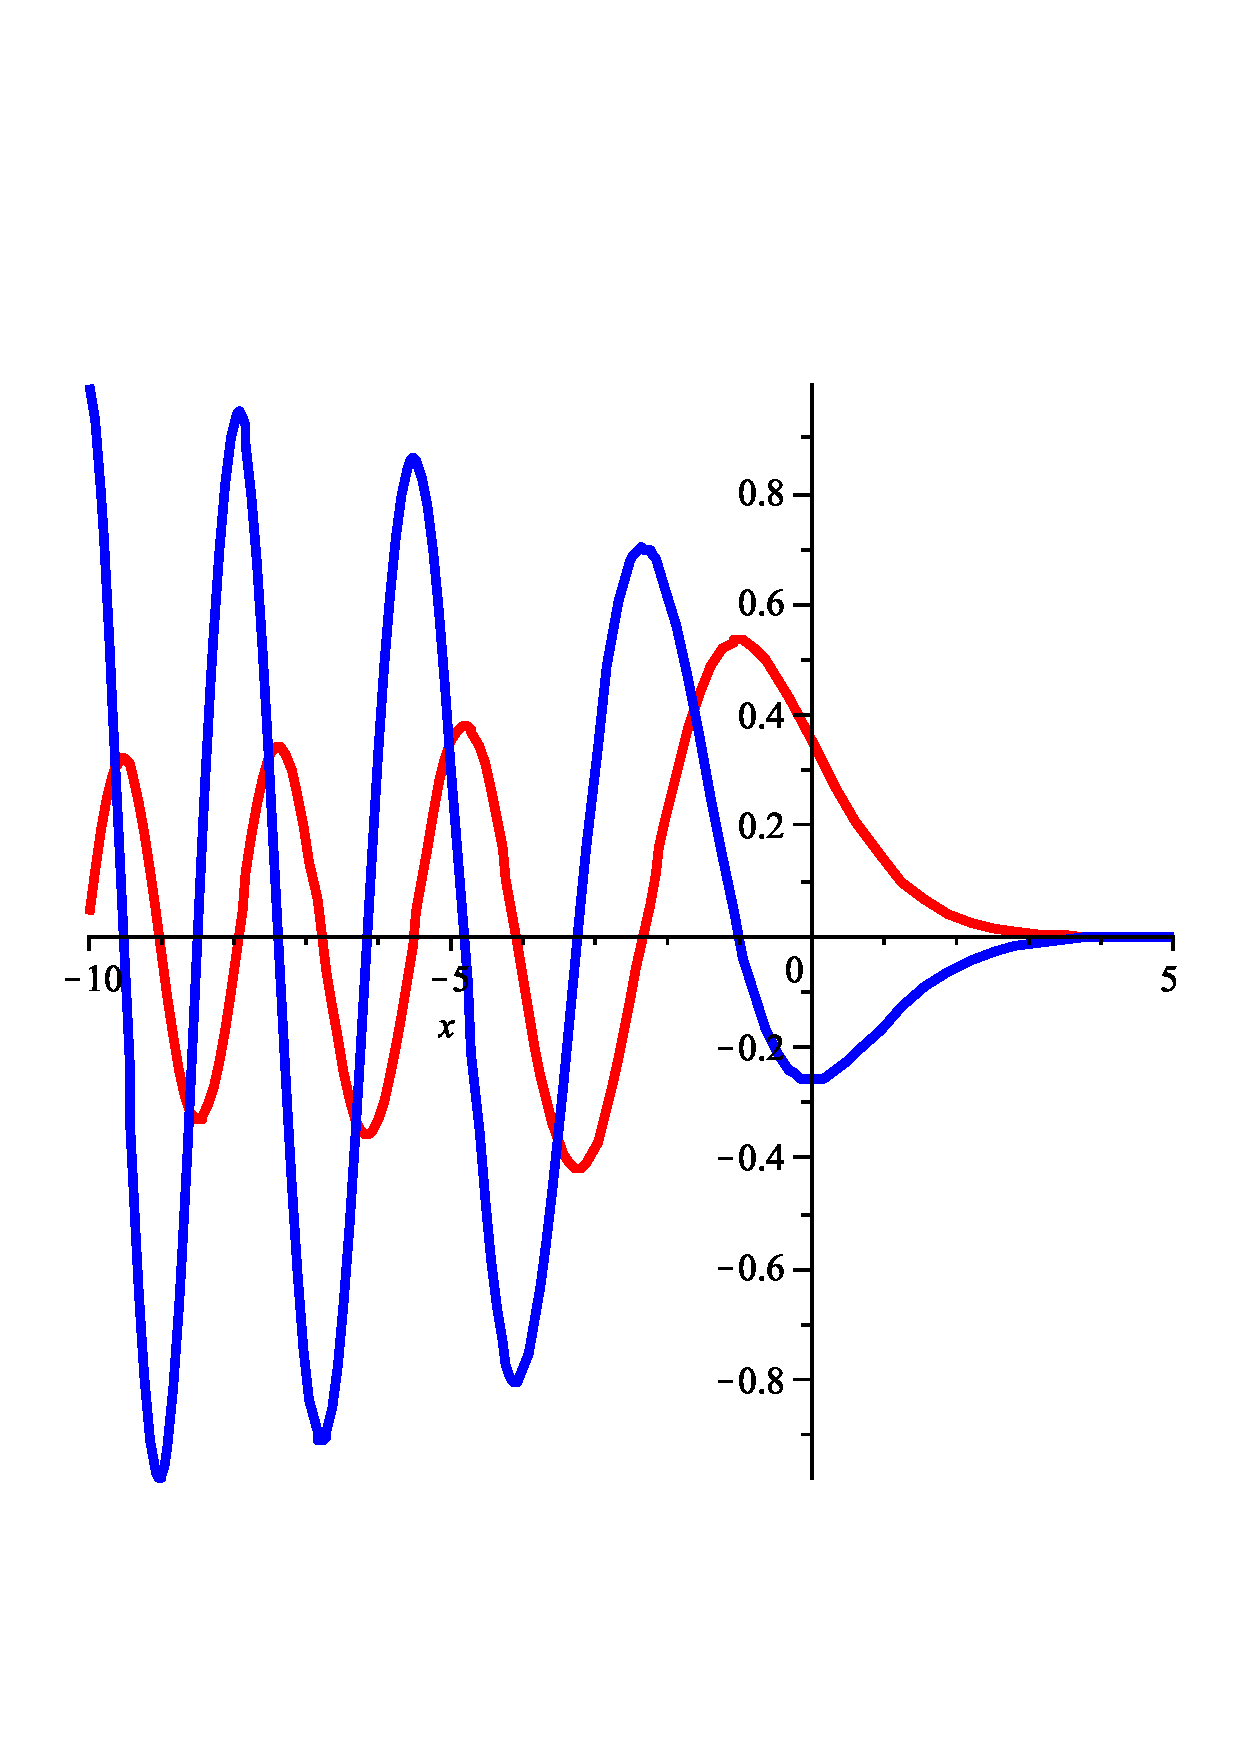
\includegraphics[scale=0.3]{Airyplot}
\caption{Dit is de grafiek van de Airyfunctie (in rood) 
en haar  afgeleide (in blauw).}
\end{figure}

\end{document}

